\section{Experimental Setup}

To evaluate our methodology on a real platform, we applied it to a hexrotor with the Odroid-U3 as a computation platform, running the Robot Operating System (ROS) \cite{ROS288} in Ubuntu. For the evaluation, the hexrotor is tasked with repeatedly following a given circular trajectory.
As can be seen in Fig.~\ref{fig:time_ecdf}, the visual odometry algorithm can occcasionaly take a long time to give a pose estimate. In our formulation %in section \ref{robustMPC} 
we have assumed that the estimator satisfies the $(\delta, \epsilon)$ contract requested by the controller. Thus, to ensure that the estimator fulfills the contract and that the mathematical guarantees provided by our RAMPC formulation hold, instead of using the visual odometry algorithm to fly the robot, 
we injected delays and errors into the measurements from Vicon, which is a high accuracy localization system. 
These delays and errors were selected from the $\Delta$ curve obtained by profiling the SVO algorithm (see Section \ref{sec:Profiling_SVO}).
The hexrotor flies using these pose estimates and our RAMPC Algorithm for both the position control and setting the time deadline for the next estimate. 
The RAMPC has the positions and velocities in the 3-axes as its states ($x$), and generates control inputs in the form of desired thrust, roll and pitch (yaw is set to 0) in order to compute a given reference $x_{ref}(t)$ for a low-level controller to track. 
The RAMPC is coded in CVXGEN \cite{cvxgen} and the generated C Code is integrated in the ROS module for position control of the hexrotor, running at 20Hz. 
The sets $\ZSet_j$ are done offline in MATLAB and then used in CVXGEN as Polyhedron type constraints. 
The constraint set $X$ defines a safe set of positions and velocities in the flying area. 
The constraint set $\inpSet$ of inputs keeps desired pitch and roll magnitudes less than $30$ degrees and desired thrust within limits of the hex-rotor abilities.
%For the contract based perception and estimation algorithm we use the FAST corner detector (as in section \ref{}) providing measurements to an Unscented Kalman Filter that also uses measurements from an Inertial Measurement Unit (IMU) to provide a state estimate for the control algorithm to use.
Later in this section we show that our approach dynamically schedules different modes of the contract-based perception and estimation algorithm at run-time and also controls the dynamical system in an energy-efficient way while providing good tracking performance. 
In the evaluation subsection we will compare our results to a baseline Model Predictive Control algorithm that does not leverage co-design and operates at a fixed $\de$ mode of the perception/estimation algorithm.

%\todo[author=KM,inline]{Do we want an architecture diagram of the way the hexrotor is controlled using ROS?}
%\todo[author=YVP,inline]{Yes, the trajectory generator to MPC/RAMPC to low level part would be good to show and make for a nice fig.}
%The control performance, as measured by a function that factors in the error in following the flight path and the cost of control, is shown in Fig.~\ref{fig:CostAndModes}.
%(The details of this cost function are given in Section \ref{formulation}).


\begin{figure}[t]
	\centering
	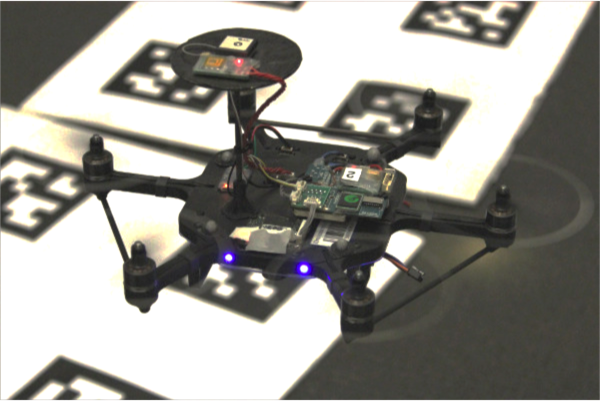
\includegraphics[width=0.7\linewidth]{figures/nanohex2}
	\caption{Autonomous hexrotor with downward-facing camera flying over synthetic features.}
	\label{fig:nanohex}
	\vspace{-10pt}
\end{figure}


\subsection{Profiling the perception and estimation pipeline}
\label{sec:Profiling_SVO}



Recall that the control algorithm needs the profiled $\Delta$ curve for the estimator. 
In our experimental setup, the estimator is given by the SVO algorithm. 
Fig. \ref{fig:svo_error_delay} shows the bound on estimation error and the $90^{th}$ percentile execution times.
This is obtained by varying the maximum number of corners knob in SVO, denoted by $\#C$, and flying extensively over a relatively feature-rich environment for each value of the knob (Fig. \ref{fig:nanohex}). 
The estimation error is computed using ground truth position obtained through the Vicon motion capture system. 
We profiled the performance for the same trajectory with different settings of the odometry offline by logging images and IMU data in-flight, and then running the visual odometry code on the Odroid-U3 offline.
This accurately recreates the in-flight environment that is present for the visual odometry algorithm and this profiling is then used online for making in-flight decisions by the control algorithm.


\begin{figure}[htb]
\centering
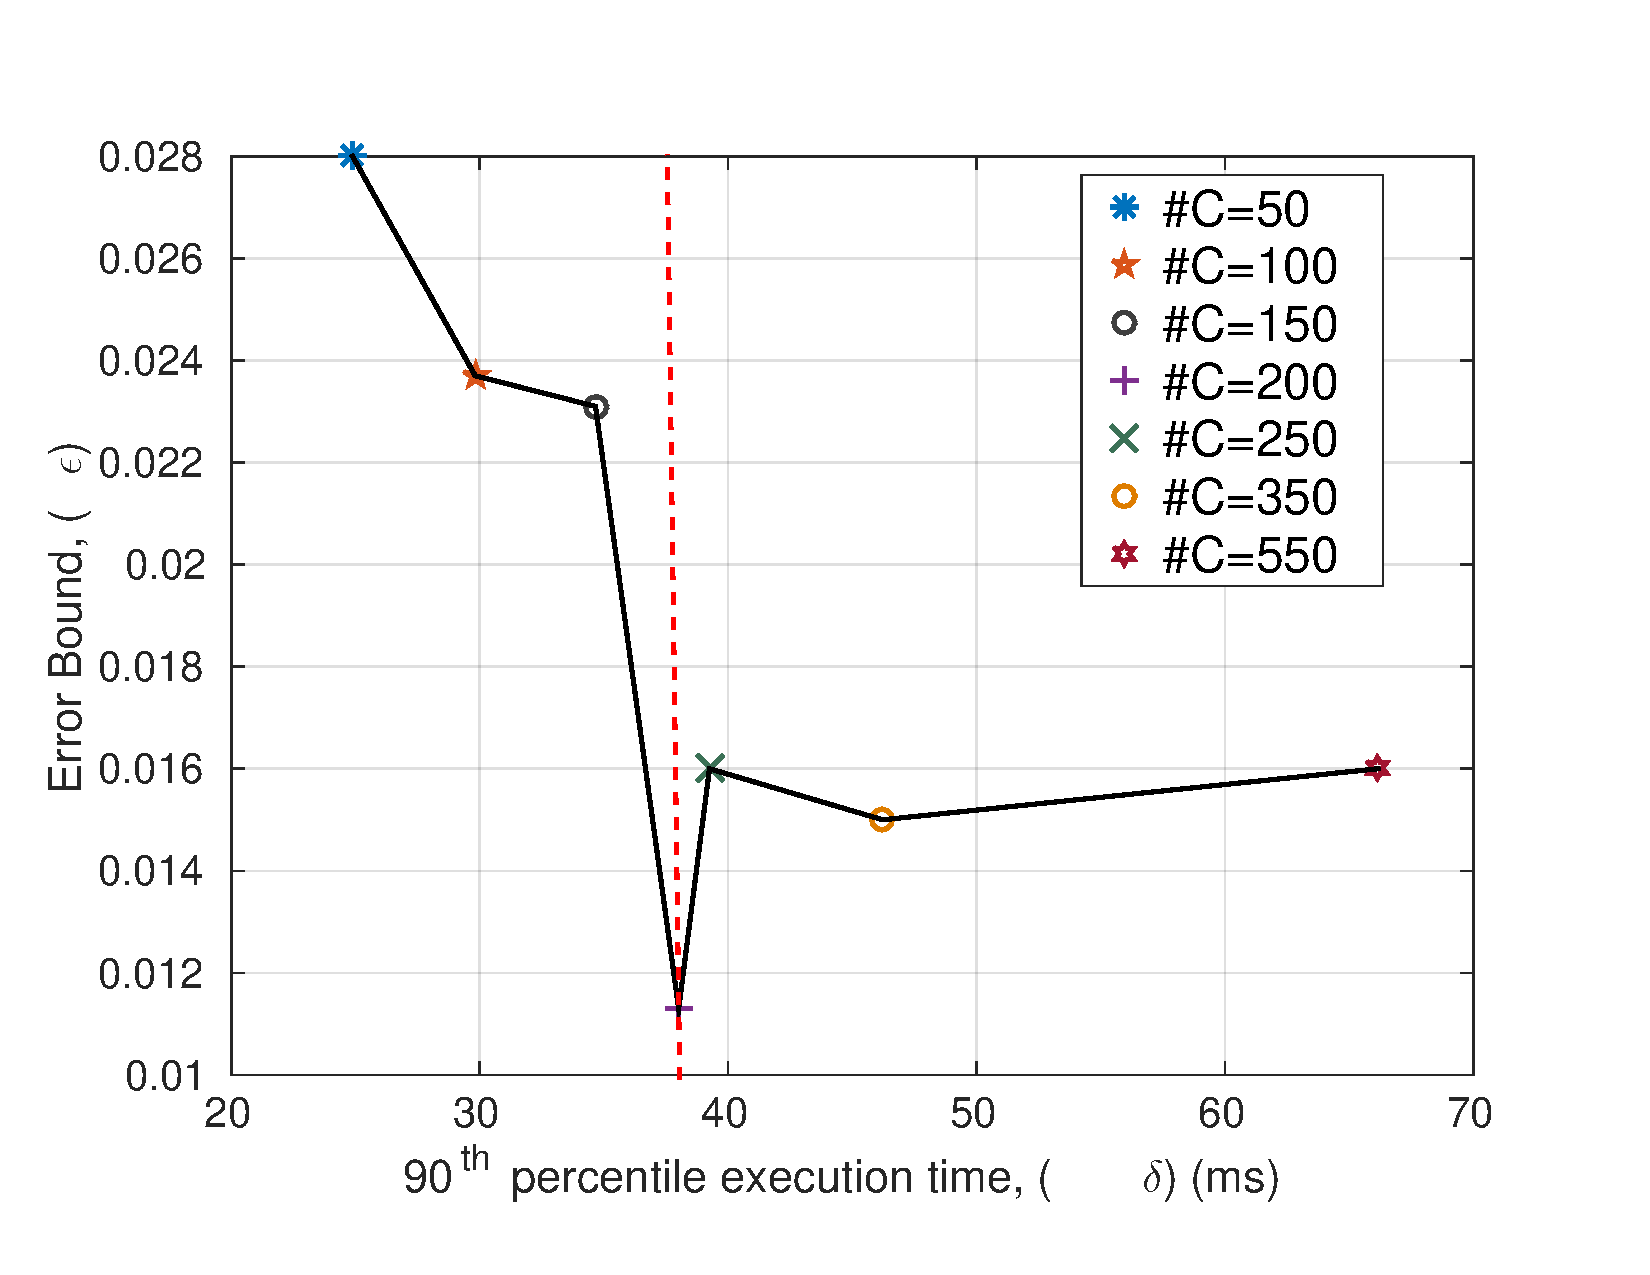
\includegraphics[width=0.99\columnwidth]{figures/errVsTime}
\vspace{-10pt}
\caption{Error-delay curve for the SVO algorithm running on the Odroid-U3 with different settings of maximum number of features ($\#C$) to detect and track. The vertical line shows the cut-off for maximum delay and the SVO settings that are allowable for closed loop control of a hexrotor at 20Hz.}
\label{fig:svo_error_delay}
\vspace{-10pt}
\end{figure}


Also needed for the control optimization %in Eq. \ref{eq:tractableOptim} 
is a measure of the power consumption by SVO at different values of the knob $\#C$. 
Power measurements are made using the Odroid Smart Power meter \cite{OdroidSmartPower}, which measures consumption at 10Hz to milliwatt precision. 
To avoid the physical challenges of fitting the power meter onto our hexrotor platform, we measure the power consumption of the Odroid board on the ground, running the same controller and vision workloads as it does during flight as explained above, and at different knob settings.
We measure the power consumption of the entire Odroid board, including CPU and DRAM power consumption. 
Since the profiling of power is done offline with other peripherals plugged into the odroid (e.g. a monitor and keyboard), we measure the idle power of the Odroid and subtract that from the power measurements when the SVO algorithm is running on it in different modes. 
This gives us a more accurate measure of the workload that the visual odometry task is responsible for. 
This offline profiling now allows us to formulate the co-design problem for the hexrotor and experimentally evaluate our methods.


\begin{figure}[htbp]
  \centering
  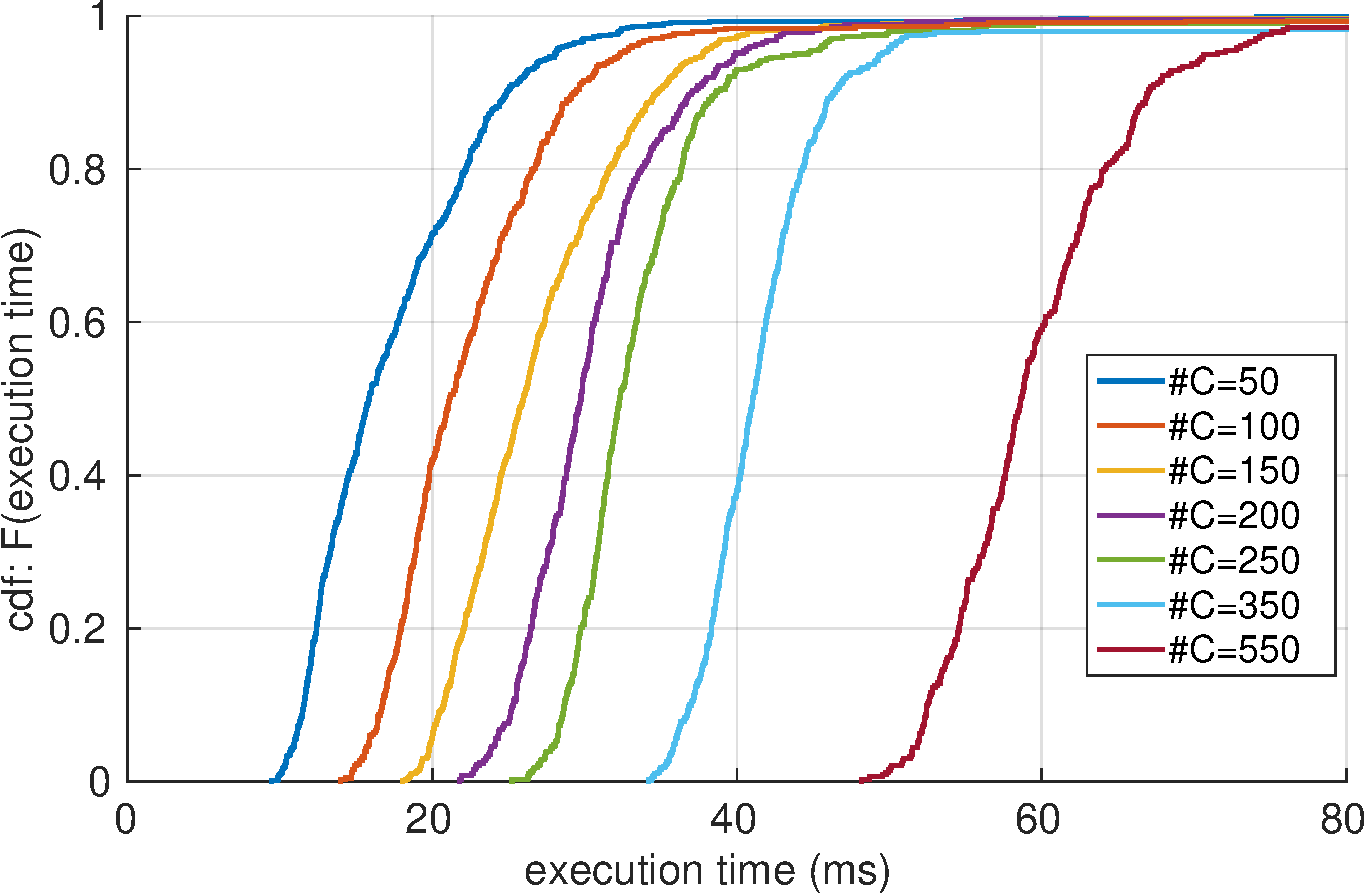
\includegraphics[width=0.9\columnwidth]{figures/time_ecdf_millisec.pdf}
  \caption{Cumulative distribution of profiled execution times for visual odometry running on the Odroid-U3 for varying maximum number of corners from the SVO algorithm.}
  \label{fig:time_ecdf}
\end{figure}